\Chapter{GTFS-adatbázisok}

A GTFS (General Transit Feed Specification) egy olyan nemzetközi szabvánnyá vált formátum, amelyben együtt kezelhetőek a tömegközlekedési menetrendek és a hozzájuk kapcsolódó földrajzi információk \cite{gtfs}, \cite{gtfsspec}.

Strukturált, szöveges állományok tartalmazzák az adatokat, amik lényegében egy adatbázis-szerkezetet definiálnak. Ezek CSV-fájlok \texttt{.txt} kiterjesztéssel egy \texttt{.zip} fájlba csomagolva. Mindegyik CSV-fájl egy adatbázistáblának felel meg, a fájl neve pedig a tábla nevét jelenti.

Az egyes táblák és a köztük lévő kapcsolatokat mutatja \aref{fig:gtfs}. ábra.

%\begin{figure}[htb]
%\centering
%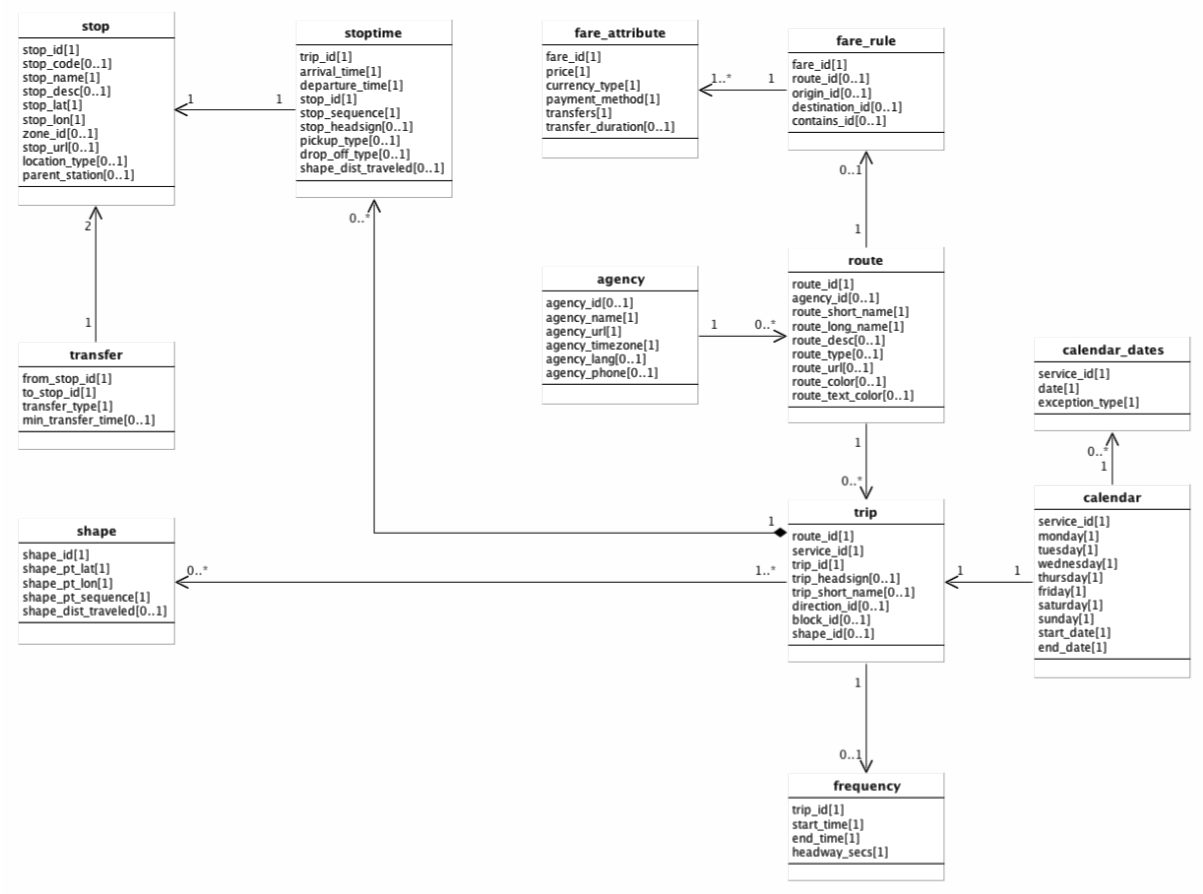
\includegraphics[scale=0.3]{kepek/gtfs_relationships.png}
%\caption{A GTFS-adatbázis tábláinak sémái és a közöttük lévő kapcsolatok.}
%\label{fig:gtfs}
%\end{figure}

\begin{figure}
\centering
\includesvg[width=400pt]{kepek/gtfs}
\caption{A GTFS-adatbázis tábláinak sémái és a közöttük lévő kapcsolatok.}
\label{fig:gtfs}
\end{figure}

A GTFS-formátum kötelező és opcionális táblákat egyaránt tartalmaz. A kötelező táblák létrehozása és adatokkal való feltöltése mindenképp szükséges a rendszer működéséhez.

\Section{Kötelező táblák}

\SubSection{agency}

A tömegközlekedési hálózat üzemeltetőjéről tartalmaz információkat. Több rekord is megadható, ha a járatokat több vállalat is üzemelteti. A route táblában minden viszonylatra meg lehet adni, hogy ki az üzemeltetője.

Kötelező mezők:

\begin{tabular}{|p{3cm}|p{10cm}|}
\hline
agency\_name & Az üzemeltető vállalt teljes neve. \\
\hline
agency\_url & A vállalat URL címe. \\
\hline
agency\_timezone & Az időzónát tartalmazza, ahol a vállalat található. \\
\hline
\end{tabular}

\SubSection{routes}

Az aktuálisan elérhető viszonylatokat tartalmazza. Minden viszonylat rendelkezik egy azonosítóval, egy rövid és egy hosszú névvel, valamint a viszonylat típusának az azonosítójával.
Kötelező mezők:

\begin{tabular}{|p{3cm}|p{10cm}|}
\hline
route\_id & Elsődleges kulcs, a viszonylat azonosítója. \\
\hline
route\_short\_name & A viszonylat rövid neve (száma). \\
\hline
route\_long\_name & A viszonylat hosszú neve, általában a két végállomást tartalmazza. \\
\hline
route\_type & Típusazonosító, lehetséges értékek:
0: villamos
1: metró
2: vasút
3: autóbusz
4: komp
5-7: egyéb járművek \\
\hline
\end{tabular}

\SubSection{trips}

Ez a tábla tartalmazza a járatokat. Mindegyik egy viszonylathoz tartozik, a direction\_id mezőben adható meg, hogy melyik irányban közlekedik a járat az adott viszonylaton (0 vagy 1 értékkel). Kötelező megadni még egy service\_id-t, ami alapján be lehet azonosítani, hogy a járat mely napokon közlekedik. Egy járathoz tartozhat még egy shape is, amely GPS koordináták sorozataként a járat útvonalát tartalmazza.
Kötelező mezők:

\begin{tabular}{|p{3cm}|p{10cm}|}
\hline
trip\_id & Elsődleges kulcs, a járat azonosítója. \\
\hline
route\_id & Idegen kulcs, a viszonylatra hivatkozik, amelyen a járat közlekedik. \\
\hline
service\_id & Idegen kulcs, a calendar és a calendar\_dates táblákra hivatkozik, ennek segítségével adható meg, hogy a járat mely napokon közlekedik. \\
\hline
\end{tabular}

\SubSection{stops}

Az egyes megállókat tárolja névvel és földrajzi koordinátákkal.
Kötelező mezők:

\begin{tabular}{|p{3cm}|p{10cm}|}
\hline
stop\_id & Elsődleges kulcs, a megálló azonosítója. \\
\hline
stop\_name & A megálló neve. \\
\hline
stop\_lat & A megálló szélességi fokát tartalmazza. A megadott értéknek WGS 84 szabvány szerintinek kell lenni. \\
\hline
stop\_lon & A megálló hosszúsági fokát tartalmazza. A megadott értéknek WGS 84 szabvány szerintinek kell lenni. \\
\hline
\end{tabular}

\SubSection{stop\_times}

Ez a tábla azt tárolja, hogy egy viszonylat egy járata egy megállóba mikor érkezik meg, mikor indul el onnan, és ez hányadik megállója az adott járatnak.
Kötelező mezők:

\begin{tabular}{|p{3cm}|p{10cm}|}
\hline
stop\_id & Idegen kulcs, a megálló azonosítója. \\
\hline
trip\_id & Idegen kulcs, a járat azonosítója. \\
\hline
arrival\_time & Érkezési idő, a járat mikor érkezik meg a megállóba. HH:MM:SS formátumban kell megadni. \\
\hline
departure\_time & Indulási idő, a járat mikor indul a megállóból. HH:MM:SS formátumban kell megadni. \\
\hline
stop\_sequence & Azt tartalmazza, hogy hányadik megállója ez a járatnak. Nemnegatív egésznek kell lennie. \\
\hline
\end{tabular}

\SubSection{calendar}

Itt úgynevezett szolgáltatásokat lehet megadni. Egy szolgáltatás azt mondja meg, hogy a járatok, amelyek ehhez a szolgáltatáshoz tartoznak, a hét mely napjain közlekednek. Továbbá meg kell adni egy érvényességi intervallumot is.
Kötelező mezők:

\begin{tabular}{|p{3cm}|p{10cm}|}
\hline
service\_id & Elsődleges kulcs, a szolgáltatás azonosítója. \\
\hline
Monday & Azt mondja meg, hogy az adott napon közlekedik-e a járat.
Az értéke lehet:
0, ha az adott napon nem közlekedik, és
1, ha az adott napon közlekedik a járat.
Tuesday

Wednesday

Thursday

Friday

Saturday

Sunday\\
\hline
start\_date & A szolgáltatás kezdő érvényességi ideje. Az értéket YYYYMMDD formátumban kell megadni. \\
\hline
end\_date & A szolgáltatás érvényességi idejének a vége. Az értéket YYYYMMDD formátumban kell megadni. \\
\hline
\end{tabular}

Opcionális táblák:

\SubSection{shapes}

A járatok útvonalát tartalmazza a tábla. Egy útvonal több pontból áll, amelyek ugyanazzal a shape\_id-val vannak ellátva.
Kötelező mezők:

\begin{tabular}{|p{3cm}|p{10cm}|}
\hline
shape\_id & Az útvonal azonosítója. \\
\hline
shape\_pt\_lat & Az útvonal egy pontjának szélességi fokát tartalmazza. A megadott értéknek WGS 84 szabvány szerintinek kell lenni. \\
\hline
shape\_pt\_lon & Az útvonal egy pontjának hosszúsági fokát tartalmazza. A megadott értéknek WGS 84 szabvány szerintinek kell lenni. \\
\hline
shape\_pt\_sequence & Azt tartalmazza, hogy hányadik pontja ez a útvonalnak. Nemnegatív egésznek kell lennie. \\
\hline
\end{tabular}

\SubSection{calendar\_dates}

A táblának két felhasználási módja van.
Ajánlott: A calendar táblával együttesen, ilyenkor a normál menetrend szerinti kivételes eseteket kell itt megadni.
Alternatív: A calendar táblát kihagyva, csak ezt a táblát használni, az összes szolgáltatást itt megadva. 
Kötelező mezők:

\begin{tabular}{|p{3cm}|p{10cm}|}
\hline
service\_id & A szolgáltatás azonosítója. Egy (service\_id, date) páros csak egyszer szerepelhet. \\
\hline
date & Egy dátumot tartalmaz, formátuma: YYYYMMDD. \\
\hline
exception\_type & Lehetséges értékei:
1, ha a szolgáltatást hozzá akarjuk adni az adott naphoz, és
2, ha a szolgáltatást el szeretnék távolítani a megadott napon. Például: ha egy járat közlekedik hétfőnként, de egy ünnep hétfőre esik, így tudjuk megadni, hogy aznap a járat nem közlekedik. \\
\hline
\end{tabular}

\SubSection{fare\_attributes}

A különböző viteldíjtípusok megadására szolgál.
Kötelező mezők:

\begin{tabular}{|p{3cm}|p{10cm}|}
\hline
fare\_id & A viteldíj azonosítója. \\
\hline
price & A viteldíj ára a currency\_type mezőben meghatározott egységben kifejezve. \\
\hline
currency\_type & A valuta ISO 4217 szabvány szerinti kódja. \\
\hline
payment\_method & Azt határozza meg, hogy a viteldíjat mikor kell kifizetni.
Lehetséges értékei:
0, ha felszálláskor kell fizetni, és
1, ha felszállás előtt kell fizetni. \\
\hline
transfers & Azt specifikálja, hogy hány átszállás lehetséges az adott viteldíjtípussal.
Lehetséges értékei:
0: nem engedélyezett az átszállás
1: egy átszállás engedélyezett
2: két átszállás engedélyezett
üres: ha a mező üres, akkor bármennyi átszállás engedélyezett. \\
\hline
\end{tabular}

\SubSection{fare\_rules}

A táblával megadható, hogy a fare\_attributes táblában található viteldíjak hogyan vonatkozzanak az útvonalakra.
Kötelező mező:

\begin{tabular}{|p{3cm}|p{10cm}|}
\hline
fare\_id & Idegen kulcs, a viteldíjat azonosítja. \\
\hline
\end{tabular}

Opcionális mezők:

% TODO: Az utolsó három jobb oldali mező össze van vonva!

\begin{tabular}{|p{3cm}|p{10cm}|}
\hline
route\_id & Idegen kulcs, a viszonylat azonosítója. Ha több viszonylathoz is ugyanaz a viteldíj tartozik, akkor minden egyes viszonylatot külön rekordként kell felvinni a táblában. \\
\hline
origin\_id & Idegen kulcsok, a stops tábla zone\_id mezőire hivatkozhatnak. \\
\hline
destination\_id &  \\
\hline
contains\_id & \\
\hline
\end{tabular}

\SubSection{frequencies}

Ha egy járat szerepel ebben a táblában, akkor az útvonaltervező figyelmen kívül hagyja a stop\_times tábla arrival\_time és departure\_time mezőjét. Ehelyett a stop\_times tábla a megállók sorrendjét és az egyes megállók közötti időkülönbséget határozza meg.
Kötelező mezők:

\begin{tabular}{|p{3cm}|p{10cm}|}
\hline
trip\_id & Idegen kulcs, egy járatra hivatkozik. \\
\hline
start\_time & Az az időpont, amikor az első jármű elhagyja a járat első megállóját. \\
\hline
end\_time & Az az időpont, amikor a járat egy másik gyakoriságra vált. \\
\hline
headway\_secs & Másodpercekben kifejezve, hogy a start\_time és az end\_time mezők által meghatározott időintervallumon belül mennyi idő telik el két indulás között ugyanabból a megállóból. \\
\hline
\end{tabular}

\SubSection{transfers}

Útvonaltervezők általában az átszállási pontokat az egyes viszonylatok megállóinak a távolságai alapján számítják ki. Az esetlegesen kétértelmű megálló párok egyértelműsítésére vagy egy konkrét csatlakozási lehetőség megadására szolgál ez a tábla.
Kötelező mezők:

\begin{tabular}{|p{3cm}|p{10cm}|}
\hline
from\_stop\_id & Idegen kulcs. Egy megálló azonosítóját tartalmazza, ahol a viszonylatok közti kapcsolat kezdődik.  \\
\hline
to\_stop\_id & Idegen kulcs. Egy megálló azonosítóját tartalmazza, ahol a viszonylatok közti kapcsolat végződik. \\
\hline
transfer\_type & A két megálló (from\_stop\_id, to\_stop\_id) közti kapcsolat típusát adja meg.
Lehetséges értékek:
0 vagy üres: Ajánlott átszállási pont a viszonylatok között.
1: Időzített átszállási pont két viszonylat között. Az induló jármű megvárja az érkezőt, elegendő időt biztosítva az utasok számára az átszálláshoz.
2: Az átszállás biztosításához bizonyos idő szükséges. Az ehhez szükséges időt a min\_transfer\_time mező tartalmazza.
3: Az adott helyen átszállás nem lehetséges a viszonylatok között. \\
\hline
\end{tabular}

\SubSection{feed\_info}

Ez a tábla az adatokat publikáló szervezetről tartalmaz információkat. Abban az esetben van fontosabb szerepe, ha a tömegközlekedési hálózat üzemeltetője és az adatok publikálója nem ugyanaz a szervezet.
Kötelező mezők:

\begin{tabular}{|p{3cm}|p{10cm}|}
\hline
feed\_publisher\_name & Az adatokat szolgáltató szervezet teljes neve. Általában megegyezik az agency tábla agency\_name mezőével. \\
\hline\
feed\_publisher\_url & Az adatokat szolgáltató szervezet URL címe. Általában megegyzik az agency tábla agency\_url mezőével. \\
\hline
feed\_lang & A szövegek alapértelmezett nyelvének IETF BCP 47 nyelvkódját tartalmazza. \\
\hline
\end{tabular}

\Section{GTFSDB}

A nyers GTFS-adatok feldolgozásához először a Google TransitFeed modulját kezdtem el használni. Ennek segítségével a memóriába be tudtam tölteni az adatokat, amiknek a lekérdezésére és a módosítására is lehetőség volt. Azonban hamar arra a következtetésre jutottam, hogy ez számomra nem lesz tökéletesen megfelelő, hiszen én mindenféleképpen adatbázisban szeretném tárolni az adatokat. A Google által kifejlesztett API segítségével is lehet az adatokat lekérdezni és módosítani, azonban úgy gondoltam, hogy az adatbázisban történő tárolással több és jobb lehetőség nyílik erre. A másik ok, amiért erre a következtetésre jutottam, hogy az adatokat ezáltal perzisztensen tudom tárolni.

Elkezdtem ilyen megoldás után kutakodni, így találtam rá az OpenTransitTools GTFSDB nevű könyvtárára. A projekt célja, hogy a GTFS-adatokat programozható kontextusba helyezze szoftverfejlesztők számára. Ennek igen nagy létjogosultsága van, hiszen a GTFS-adatokkal foglalkozó alkalmazások készítésénél általában az első lépés a nyers adatok lekérdezhetővé, feldolgozhatóvá tétele. A GTFSDB könyvtár segítségével PostgreSQL, Oracle, MySQL és SQLite adatbázisokat hozhatunk létre a nyers adatokból. A projekt forráskódja elérhető GitHubon: https://github.com/OpenTransitTools/gtfsdb

\begin{python}
path = resource_filename('gtfsdb', 'zips')
gtfs_file = 'file:///{0}'.format(os.path.join(path, 'mvkzrt.zip'))
basedir = os.path.abspath(os.path.dirname(__file__))
url = 'sqlite:///' + os.path.join(basedir, 'mvk.db')
db = database_load(gtfs_file, url=url)
\end{python}

Az adatbázis létrehozása és feltöltése a database\_load függvény meghívásával történik. Paraméterként meg kell adni a GTFS-adatokat tartalmazó \texttt{.zip} fájlt, illetve a létrehozni kívánt adatbázisfájl helyét, nevét és típusát. Ezt lefuttatva létrejönnek a táblák és feltöltődnek adatokkal. Ez után már SQLAlchemy segítségével könnyedén lekérdezhetővé válnak az adatok.

A GTFSDB-t Python 2.7-es verzióval ajánlott használni, így először én is azzal próbáltam. Ezáltal viszont a következő problémába ütköztem bele. Az adatbázis feltöltése közben hiba keletkezett, nem sikerült az ékezetet tartalmazó szövegek feldolgozása. Témavezetőm azt tanácsolta, hogy próbáljam meg a Python 3-as verziójával lefuttatni a kódot, és akkor valószínűleg az ékezetes betűkből adódó karakterkódolási hiba meg fog szűnni. Ahhoz, hogy a GTDSDB működjön Python 3-mal, ahhoz a forráskódjában néhány sort át kellett írni. A következőkben ezeket a változtatásokat ismertetem.

gtfsdb/config.py

1. sor:
\begin{python}
-from ConfigParser import ConfigParser
+from configparser import ConfigParser
\end{python}

gtfsdb/model/base.py

33. sor:
\begin{python}
-except Exception, e:
+except Exception as e: 
\end{python}

158. sor:
\begin{python}
-if isinstance(v, basestring):
+if isinstance(v, str):
\end{python}

171. sor:
\begin{python}
-except Exception, e:
+except Exception as e:
\end{python}

gtfsdb/model/db.py

82. sor:
\begin{python}
-except Exception, e:
+except Exception as e:
\end{python}

gtfsdb/model/gtfs.py

6. sor:
\begin{python}
-from urllib import urlretrieve
+from urllib.request import urlretrieve
\end{python}

53. sor:
\begin{python}
-except Exception, e:
+except Exception as e:
\end{python}

gtfsdb/model/route\_stop.py

260. sor:
\begin{python}
-print unique_stops
+print(unique_stops)
\end{python}

gtfsdb/model/stop\_time.py

75. sor:
\begin{python}
-except Exception, e:
+except Exception as e:
\end{python}

Ezekkel a változtatásokkal, Python 3 alatt, sikeresen lefutott a database\_load függvény ékezetes karaktereket tartalmazó forrásfájlok esetén is.

